\documentclass[12pt, titlepage, a4paper]{article}

\usepackage{cmap}
\usepackage[utf8]{inputenc}
\usepackage[T1]{fontenc}
\usepackage[czech]{babel}
\usepackage{listings}
\usepackage{xcolor}
\usepackage{pdfpages}
\usepackage[top=3cm, bottom=3cm, left=2.5cm, right=2.5cm]{geometry}

\definecolor{light-gray}{gray}{0.90}
\definecolor{gray}{rgb}{177,179,181}
\definecolor{codegreen}{rgb}{0,0.6,0}
\definecolor{codegray}{rgb}{0.5,0.5,0.5}
\definecolor{codepurple}{rgb}{0.58,0,0.82}
\definecolor{backcolour}{rgb}{0.95,0.95,0.92}

\lstdefinelanguage{JavaScript}{
  morekeywords={typeof, new, true, false, catch, function, return, null, catch, switch, var, if, in, while, do, else, case, break},
  morecomment=[s]{/*}{*/},
  morecomment=[l]//,
  morestring=[b]",
  morestring=[b]'
}

\lstset{
    language=[Sharp]C,
    breaklines=true,
    breakatwhitespace=true,
    xleftmargin=10pt,
    % numbers=left,
    numberstyle=\tiny\color{codegray},
    commentstyle=\color{codegreen},
    keywordstyle=\color{blue},
    backgroundcolor = \color{light-gray},
    showstringspaces=false
}

\begin{document}
    \begin{titlepage}
        \bfseries{
            \begin{center}
                \Large{DELTA – Střední škola informatiky a ekonomie, Základní škola a Mateřská škola
                s.r.o.
                \newline
                Ke Kamenci 151, PARDUBICE}
                \vspace{0.4 \textheight}\\
                \large{
                    MATURITNÍ PROJEKT
                }\\
                \vspace{14pt}
                \LARGE{
                    Řešení vybraných problémů algoritmiky grafů
                }
                \vspace{0.3 \textheight}
            \end{center}
        \noindent\large{Martin Klíma}\\
        \noindent\large{4.B}\\
        \noindent\large{Informační technologie 18-20-M/01}\\
        \noindent\large{2022/2023}\\
        }
  \end{titlepage}
\clearpage

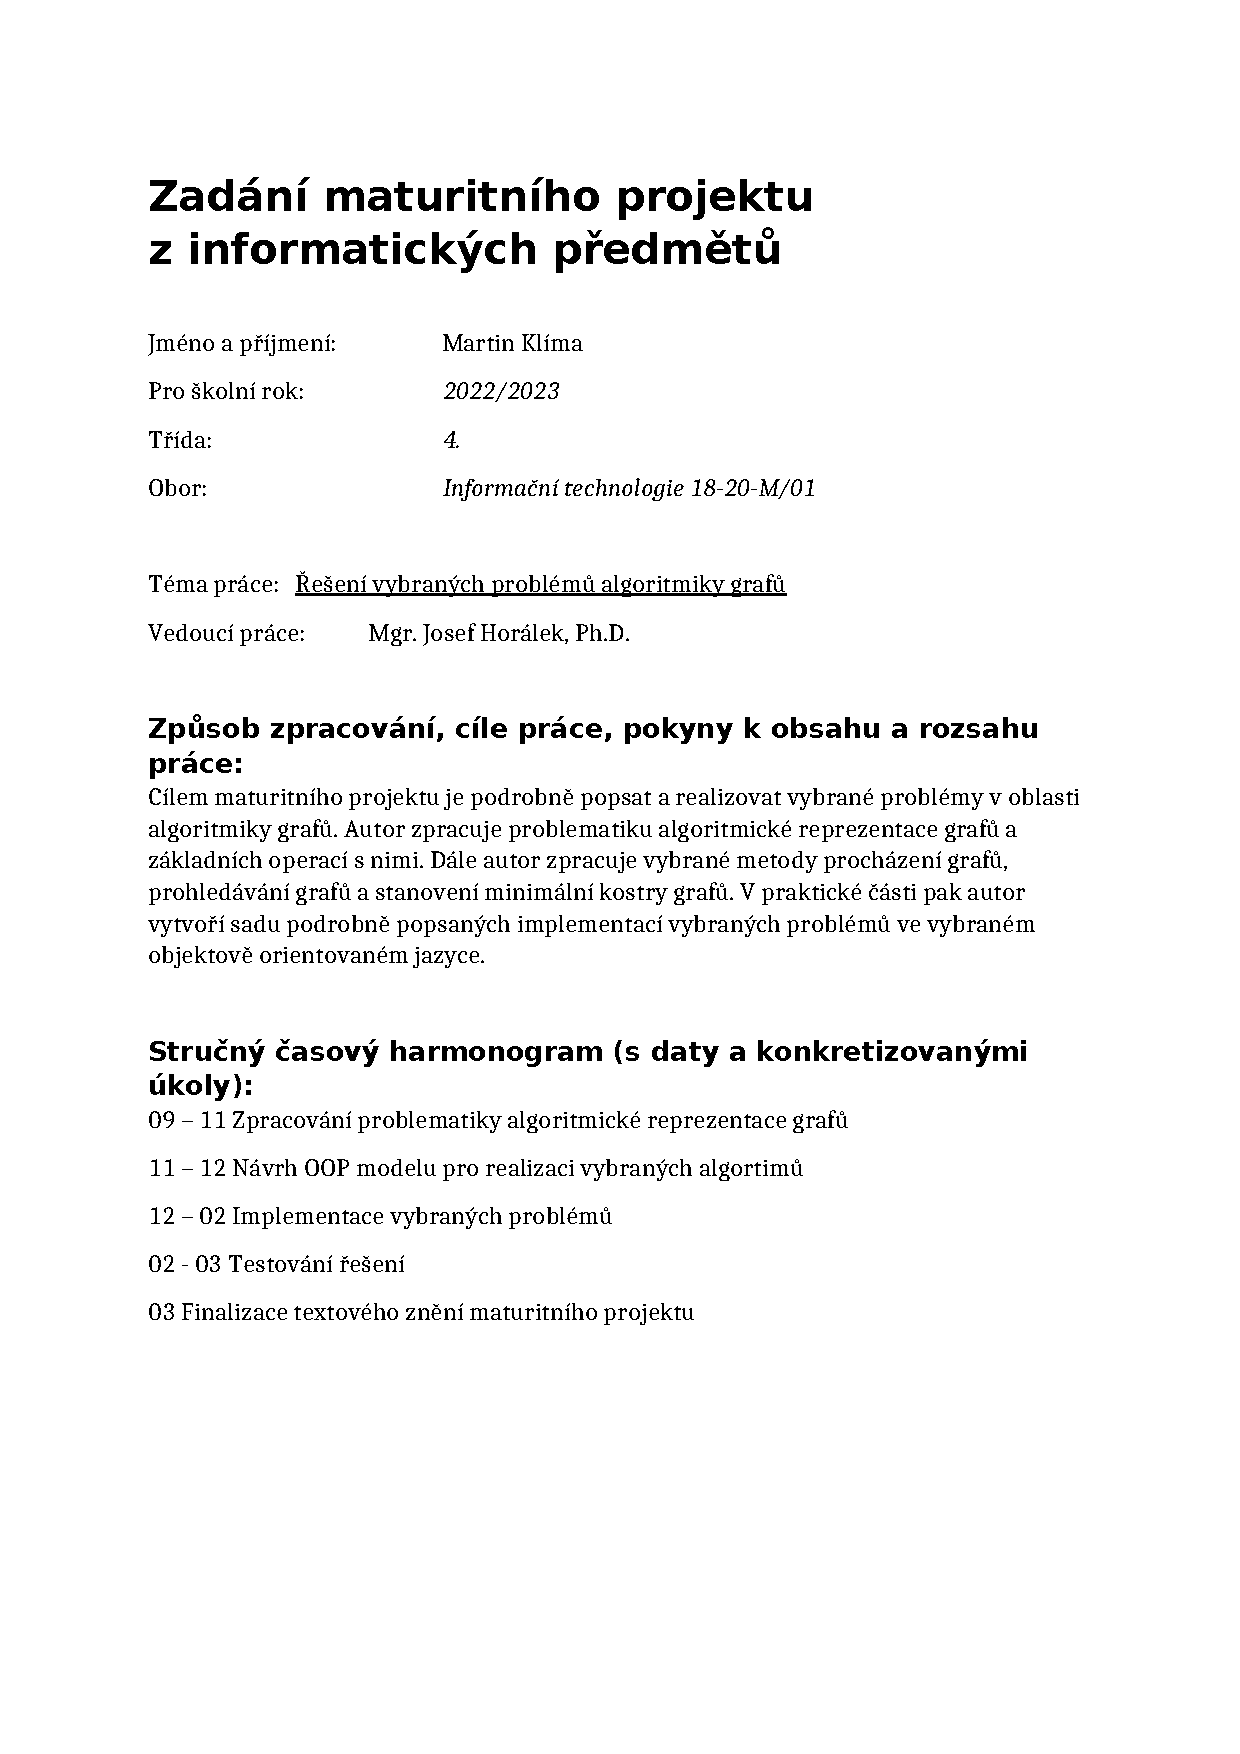
\includepdf{files/Zadani.pdf}
\clearpage
% prohlášení
\vspace*{0.8\textheight}
\noindent{\Large{\bfseries{Prohlášení}}}

\noindent{Prohlašuji, že jsem maturitní projekt vypracoval(a) samostatně, výhradně s použitím
uvedené literatury.}

\vspace{20pt}

\noindent V Pardubicích 31.3.2023 \hspace{150pt}\dotfill{}\hspace{\stretch{0.5}}

\hspace{9.5cm} Martin Klíma
\clearpage
\tableofcontents
\newpage

\section{Úvod}
\paragraph{}
Cílem maturitní práce je podrobně popsat a realizovat vybrané problémy v oblasti 
algoritmiky grafů zaměřených na prohledávání grafů.
Tento maturitní projekt bude využit jako doprovodný studijní materiál předmětu 
algoritmy, jehož cílem je seznámit studenty se základními principy 
prohledávání grafů do hloubky, do šířky a vybraných algoritmických problémů. 
Pro naplnění cílů této práce jsou teoreticky popsány principy fungování prohledávání do hloubky,
prohledávání do šírky a vyhledávání nejkratší cesty.
\paragraph{}
Praktická realizace celého projektu je navržena v programovacím jazyce javascript za pomocí svelte
, jehož kódová část je popsána jako součást dokumentace. Výstupem práce je webová stránka 
s GUI rozhraním, které umožňuje uživateli (studentovi) výběr konkrétního algoritmu s ukázkou jeho implementace.

\section{Úvod do grafů}
\paragraph{}
Grafy jsou matematické objekty, které se skládají z vrcholů a hran, které spojují tyto 
vrcholy. Grafy sou využívány jako model pro mnoho různých situací v informatice a jiných 
oblastech, jako například počítačové sítě, telekomunikace a dopravní systémy.
\paragraph{}
Jedním z nejdůležitějších problémů v algoritmice grafů je nalezení nejkratší cesty mezi 
dvěmi vrcholy. Tento problém se řeší pomocí různých algoritmů, jako například Dijkstrův 
algoritmus, Bellman-Fordův algoritmus nebo algoritmus Floyd-Warshall. Tyto algoritmy 
pracují s váženými grafy, kde každá hrana má určitou váhu (hodnotu).
\paragraph{}
Dalším důležitým problémem v algoritmice grafů je hledání minimální kostry grafu. Minimální 
kostra grafu je podgraf grafu, který obsahuje všechny vrcholy grafu a zároveň má nejmenší 
součet vah (hodnot) hran. Tento problém se řeší pomocí algoritmů jako Kruskalův algoritmus nebo Primův 
algoritmus. Minimální kostra grafu se často využivá v počítačových sítích pro zajištění redundance
a integrity v rozsáhlejších sítích za pomocí spanning tree.
\paragraph{}
Grafy jsou v informatice často používány jako model pro sítě. Sítě mohou být fyzické nebo 
logické, a grafy poskytují užitečný nástroj pro modelování a analýzu různých vlastností sítí.
\paragraph{}
Důležitou vlastností sítí je maximální tok, což je maximální množství, které může být přeneseno 
sítí mezi dvěma uzly v daném čase. Tento problém se řeší pomocí algoritmů jako Ford-Fulkersonův 
algoritmus, Edmonds-Karpův algoritmus nebo Dinicův algoritmus.
\newpage

\subsection{Depth First Search}
\subsubsection{Popis algoritmu}
\paragraph{}
Algoritmus pro procházení grafů do hloubky (anglicky Depth-First Search) dále DFS
je jedním ze základních algoritmů pro procházení grafů. Algoritmus DFS prochází 
graf postupně z jednoho vrcholu do dalších tak dlouho, dokud to bude možné. 
Pokud narazí na vrchol, který již byl navštíven, algoritmus se vrátí zpět a pokračuje 
v procházení grafu z jiného vrcholu.
~\cite{GeeksforGeeks: DFS,Khan Academy: DFS}

\subsubsection{Funkcionalita algoritmu}
\paragraph{}
Při jednom způsobu implementace algoritmu DFS se využívá zásobník (stack).Na začátku vybere jeden z vrcholů a 
následně jej uloží do již navštívených-otevřených vrcholů. Z něho pokračuje na libovolný nenavštívený vrchol, 
který následně opět přidá mezi již navštívené-otevřené vrcholy a takto pokračuje až do momentu, kdy 
z aktuálního vrcholu nevede cesta k vrcholu doposud nenavštívenému. V tento moment se využije 
backtracking a algoritmus označí aktuální vrchol za navštívený-uzavřený a posune se o jeden vrchol 
„zpět“, kde hledá cestu k nenavštívenému vrcholu. Opakováním tohoto procesu projdeme postupně 
všechny vrcholy grafu a vrátíme se do začátečního vrcholu.

\paragraph{}
Druhý způsob implementace algoritmu je za pomocí rekurze, při kterém algoritmus začne v 
počátečním vrcholu a zjistí všechny dostupné nenavštívené vrcholy. Po zjištení dostupných 
nenavštívených vrcholů je stejný proces opakován na dostupných vrcholech, dokud algoritmus 
neprojde celý dostupný graf.
~\cite{GeeksforGeeks: DFS,Khan Academy: DFS}

\subsubsection{Výhody a nevýhody algoritmu}
\paragraph{}
Algoritmus DFS je velmi jednoduchý a intuitivní, ale má několik nevýhod. Jednou z 
nevýhod je, že může být velmi pomalý pro grafy s mnoha vrcholy a hranami. Dále může 
vést k rekurzivnímu zanořování a potenciálně k překročení maximální hloubky rekurze.

\subsubsection{Využití algoritmu}
\paragraph{}
DFS algoritmus je implementován v mnoha řešeních v oblasti informatiky obsahující grafy. 
Využívá se například pro topologické uspořádání uzlu. Pokaždé, když označíme uzel za uzavřený, 
uložíme jej do zásobníků a tímto vytvoříme topologické uspořádání uzlů.
\paragraph{}
Dále se využívá například k určení acykličnosti grafu. Při prohledávání grafu můžeme kontrolovat zpětné hrany (hrany 
vedoucí do vrcholu navštíveného-otevřeného). Pokud se žádná hrana vyjma hrany příchozí 
nevyskytuje, je graf acyklický.

\newpage
\subsubsection{Implementace algoritmu}
\begin{lstlisting}
using System;
using System.Collections.Generic;

public class Program
{
    public static void Main()
    {
        // create a new stack to use in DFS
        Stack<int> stack = new Stack<int>();

        // create a new graph with 4 vertices
        Graph g = new Graph(4);

        // add edges to the graph
        g.addEdge(0, 1);
        g.addEdge(0, 2);
        g.addEdge(1, 2);
        g.addEdge(2, 0);
        g.addEdge(2, 3);
        g.addEdge(3, 3);

        // perform DFS starting from vertex 2
        g.DFS(2);
    }
}

public class Graph
{
    int V; // the number of vertices in the graph
    List<int>[] adj; // an array of adjacency lists to represent the graph

    // constructor to initialize the graph with the given number of vertices
    public Graph(int v)
    {
        V = v;
        adj = new List<int>[v];
        for (int i = 0; i < v; i++)
        {
            adj[i] = new List<int>();
        }
    }

    // method to add an edge between two vertices in the graph
    public void addEdge(int v, int w)
    {
        adj[v].Add(w);
    }

    // method to perform depth-first search starting from the given source vertex
    public void DFS(int s)
    {
        bool[] visited = new bool[V]; // array to keep track of visited vertices
        for (int i = 0; i < V; i++)
            visited[i] = false;
        Stack<int> stack = new Stack<int>(); // create a new stack for DFS
        stack.Push(s); // add the source vertex to the stack
        visited[s] = true; // mark the source vertex as visited
        while (stack.Count != 0) // loop until the stack is empty
        {
            int pop = stack.Pop(); // remove the next vertex from the stack
            Console.Write(pop + " "); // print the vertex
            foreach (var vert in adj[pop]) // iterate over the adjacent vertices
            {
                if (!visited[vert]) // if the adjacent vertex is not visited
                {
                    visited[vert] = true; // mark it as visited
                    stack.Push(vert); // add it to the stack
                }
            }
        }
    }
}
\end{lstlisting}
\clearpage

\subsection{Breadth First Search}
\subsubsection{Popis algoritmu}
\paragraph{}
Prohledávání grafu do šířky (anglicky Breadth-First Search) dále BFS je algoritmus 
pro prohledávání grafů, který postupuje systematicky a rozšiřuje průzkum postupně po 
vrstvách. Tedy nejprve navštíví všechny sousedy zdrojového vrcholu, poté všechny sousedy 
sousedů a tak dále. Algoritmus je založen na principu prohledávání grafu pomocí fronty.

\subsubsection{Funkcionalita algoritmu}
\paragraph{}
BFS začíná v zadaném vrcholu grafu a postupně prochází všechny sousedy tohoto vrcholu. 
Všechny sousední vrcholy vloží do fronty, aby je bylo možné prohledat v následujícím kroku 
a sem je uložen mezi již prohledané vrcholy. Po uložení všech sousedních vrcholů pokračuje 
algoritmus se stejným postupem na vrcholy uložené ve frontě a postupně tím frontu k vyřešení 
zkracuje tím, že již vyřešené vrcholy ukládá do fronty již zpracovaných vrcholů. Tento proces 
se opakuje, dokud jsou nacházeny nenavštívené sousední vrcholy grafu.

\subsubsection{Výhody a nevýhody algoritmu}
\paragraph{}
BFS algoritmus vyniká tím, že s jistotou najde řešení zadaného grafu, pokud je graf řešitelný.
Pokud má graf více možných řešení, BFS vždy najde řešení s nejmenším počtem kroků. Spolehlivost 
se ovšem musí odrazit na jiném aspektu algoritmu a to je jeho využití paměti. Ukládáním veškerých 
vrcholů k projití a již vyřešených vrcholů do fronty využívá BFS algoritmus více paměti oproti ostatním algoritmům
na procházení grafů. Zároveň při procházení velkých grafů může být časově náročnější.

\subsubsection{Využití algoritmu}
\paragraph{}
BFS algoritmus nalezne využití v mnoha případech jako DFS algoritmus. Jeho odlišným průchodem grafu se ovšem hodí 
pro jiná využití než prohledávání do hloubky. Využití BFS algoritmu je například v Peer to Peer sítích, kde se 
využívá pro nalezení všech sousedních uzlů, například v Torrentové síti. Další využití nalezne v sociálních sítích,
kde se používá pro nalezení známých uživatelů, kdy uživatelé reprezentují vrcholy grafu a přátelství mezi nimi hrany.
Dále je využíván při optimalizaci vyhledávačů pro indexování. Cílem je začít na zdrojové stránce a postupně prohledat 
veškeré dostupné odkazy na jiné stránky a následně opakovat pro každou nalezenou stránku. Při indexování pro vyhledávače 
lze využít i DFS algoritmus, ovšem zde se projevuje výhoda BFS algoritmu, který postupuje postupně po úrovních a tím pádem 
je možné snáze nastavit hloubku prohledávání.

\subsubsection{Implementace algoritmu}

\begin{lstlisting}
using System;
using System.Collections.Generic;

public class Graph
{
    private int V; // number of vertices in the graph
    private List<int>[] adj; // adjacency list representing the graph

    // Constructor to initialize the graph
    public Graph(int v)
    {
        V = v;
        adj = new List<int>[v];

        // Initialize each element of the adjacency list to an empty list
        for (int i = 0; i < v; i++)
        {
            adj[i] = new List<int>();
        }
    }

    // Method to add an edge between two vertices
    public void AddEdge(int v, int w)
    {
        // Add vertex w to the adjacency list of vertex v
        adj[v].Add(w);
    }

    // Method to perform BFS traversal of the graph
    public void BFS(int s)
    {
        // Create a boolean array to keep track of visited vertices
        bool[] visited = new bool[V];

        // Create a queue to store the vertices to be visited
        Queue<int> queue = new Queue<int>();

        // Mark the source vertex as visited and enqueue it
        visited[s] = true;
        queue.Enqueue(s);

        while (queue.Count != 0)
        {
            // Dequeue a vertex from the queue and print it
            s = queue.Dequeue();
            Console.Write(s + " ");

            // Get all adjacent vertices of the dequeued vertex s
            // If an adjacent vertex has not been visited, mark it as visited and enqueue it
            foreach (int i in adj[s])
            {
                if (!visited[i])
                {
                    visited[i] = true;
                    queue.Enqueue(i);
                }
            }
        }
    }
}

// Driver code to test the implementation
public class BFS
{
    public static void Main()
    {
        Graph g = new Graph(4); // Create a graph with 4 vertices

        // Add edges to the graph
        g.AddEdge(0, 1);
        g.AddEdge(0, 2);
        g.AddEdge(1, 2);
        g.AddEdge(2, 0);
        g.AddEdge(2, 3);
        g.AddEdge(3, 3);

        Console.WriteLine("BFS traversal starting from vertex 2:");
        g.BFS(2); // Perform BFS traversal starting from vertex 2
    }
}
\end{lstlisting}
\clearpage

\subsection{Dijkstrův algoritmus}
\subsubsection{Popis algoritmu}
\paragraph{}
Dijkstrův algoritmus je zaměřený na vyhledávání nejkratší cesty v váženém grafu. Algoritmus 
vyhledává nejkratší cestu ze zvoleného počátečního uzlu do všech ostatních uzlů v grafu s 
ohledem na váhu (hodnotu) hran mezi nimi. Algoritmus jepoujmenován po nizozemském vědci 
Edsgeru W. Dijkstrovi, který ho popsal v roce 1959.

\subsubsection{Funkcionalita algoritmu}
\paragraph{}
Dijkstrův algoritmus je založen na principu postupného procházení grafu, přičemž pro každý 
uzel uchovává nejkratší známou cestu z počátečního uzlu. Algoritmus se řídí principem tzv. 
"hladového algoritmu" (angl. greedy algorithm), kdy v každé iteraci vybírá z nezpracovaných 
uzlů ten s nejmenší dosud známou vzdáleností od počátečního uzlu.
\paragraph{}
Postup algoritmu je následující:
\begin{enumerate}
    \item Nejprve se inicializuje graf a počáteční uzel. Pro každý uzel se uchovává jeho 
    dosud nejkratší vzdálenost od počátečního uzlu, pro počáteční uzel se nastaví tato 
    vzdálenost na 0, zatímco pro všechny ostatní uzly se nastaví na nekonečno.

    \item Následně se vybírá nezpracovaný uzel s nejmenší dosud známou vzdáleností od 
    počátečního uzlu a zpracuje se. V této fázi se do uzlu přidávají sousední uzly, kde 
    sousední uzel je takový uzel, který je spojen hranou s aktuálním uzlem.
    
    \item Pro každý sousední uzel se zkontroluje, zda je jeho nově vypočítaná vzdálenost 
    menší než jeho dosud známá vzdálenost. Pokud ano, nová vzdálenost se uloží jako jeho 
    nejkratší vzdálenost a uzel se přidá do seznamu nezpracovaných uzlů.
    
    \item Postup se opakuje, dokud nejsou zpracovány všechny uzly, pro které existuje 
    cesta z počátečního uzlu.
\end{enumerate}
\paragraph{}
Na konci algoritmu jsou tedy pro každý uzel grafu známy jeho nejkratší vzdálenosti od 
počátečního uzlu, což umožňuje nalezení nejkratší cesty z počátečního uzlu do kteréhokoliv 
jiného uzlu v grafu.

\subsubsection{Výhody a nevýhody algoritmu}
\paragraph{}
Výhodou Dijkstrova algoritmu je jeho univerzálnost. Jelikož algoritmus nepotřebuje znát 
cílový uzel, je možné ho použít pro vyhledávání nejkratší cesty z jednoho uzlu do všech 
ostatních uzlů v grafu, proto je vhodný pro řešení úloh, kde je více cílových uzlů a je 
zapotřebí určit nejbližší uzel. Nevýhodou algoritmu je jeho nepoužitelnost pro grafy s 
negativními váhami hran.

\subsubsection{Využití algoritmu}
\paragraph{}
Djikstrlv algoritmus se využívá v navigačních systémech, kde je potřeba určit nejkratší cestu 
mezi dvěma body na mapě. Dále se využívá v systémech pro plánování letů, kde je potřeba určit 
nejkratší cestu mezi letišti. Algoritmus také nachází uplatnění v počítačových sítích, kde se 
využívá k určení nejkratší cesty mezi dvěma routery v síti pro přenos dat. Další využití 
tohoto algoritmu je ve videohrách, kde se využívá k určení trasy pro nehráčské postavy po světě.

\subsubsection{Implementace algoritmu}
\begin{lstlisting}
using System;

class GFG {
static int V = 9; // Number of vertices in the graph

// This function finds the vertex with the minimum distance value,
// from the set of vertices not yet included in shortest path tree.
int minDistance(int[] dist, bool[] sptSet)
{
    int min = int.MaxValue, min_index = -1;

    // Loop through all vertices
    for (int v = 0; v < V; v++)
        // Check if vertex v is not in sptSet and if its distance
        // from source is less than the current minimum distance
        if (sptSet[v] == false && dist[v] <= min) {
            // Update the minimum distance and the index of the vertex
            min = dist[v];
            min_index = v;
        }

    // Return the index of the vertex with the minimum distance
    return min_index;
}

// This function prints the distance of all vertices from the source
void printSolution(int[] dist)
{
    Console.Write("Vertex 		 Distance "
                  + "from Source
");
    for (int i = 0; i < V; i++)
        Console.Write(i + " 		 " + dist[i] + "
");
}

// This function implements Dijkstra's algorithm to find the shortest
// path from a source node to all other nodes in a weighted graph.
void dijkstra(int[, ] graph, int src)
{
    int[] dist= new int[V]; // Array to store the shortest distance from the source to each vertex

    bool[] sptSet = new bool[V]; // Array to store whether a vertex is included in the shortest path tree or not

    // Initialize all distances to infinity and sptSet to false
    for (int i = 0; i < V; i++) {
        dist[i] = int.MaxValue;
        sptSet[i] = false;
    }

    dist[src] = 0; // Set the distance of the source node to 0

    // Loop through all vertices except the source
    for (int count = 0; count < V - 1; count++) {
        int u = minDistance(dist, sptSet); // Find the vertex with the minimum distance from the source

        sptSet[u] = true; // Add the vertex to the shortest path tree

        // Update the distance of all adjacent vertices if the new path through
        // the current vertex is shorter than the previously known path
        for (int v = 0; v < V; v++){
            if (!sptSet[v] && graph[u, v] != 0
                && dist[u] != int.MaxValue
                && dist[u] + graph[u, v] < dist[v])
                dist[v] = dist[u] + graph[u, v];
        }
    }
    // Print the shortest distances of all vertices from the source
    printSolution(dist);
}

public static void Main()
{
    // Example graph as an adjacency matrix
    int[,] graph = new int[,] { { 0, 4, 0, 0, 0, 0, 0, 8, 0 },
                            { 4, 0, 8, 0, 0, 0, 0, 11, 0 },
                            { 0, 8, 0, 7, 0, 4, 0, 0, 2 },
                            { 0, 0, 7, 0, 9, 14, 0, 0, 0 },
                            { 0, 0, 0, 9, 0, 10, 0, 0, 0 },
                            { 0, 0, 4, 14, 10, 0, 2, 0, 0 },
                            { 0, 0, 0, 0, 0, 2, 0, 1, 6 },
                            { 8, 11, 0, 0, 0, 0, 1, 0, 7 },
                            { 0, 0, 2, 0, 0, 0, 6, 7, 0 } };
        GFG g = new GFG();
 
        // Function call
        g.dijkstra(graph, 0);
    }
}
\end{lstlisting}
\section{Aplikace}
\subsection{Využité technologie}
\begin{enumerate}
    \item Javascript
    \item Svelte
\end{enumerate}
\subsubsection{Javascript}
\paragraph{}
JavaScript je vysokoúrovňový, interpretovaný programovací jazyk používaný pro tvorbu interaktivních 
webových stránek a webových aplikací. Byl vyvinut firmou Netscape v roce 1995.
\paragraph{}
Jazyk JavaScript je objektově orientovaný, což znamená, že se v něm pracuje s objekty a metodami, 
které se používají k interakci s HTML a CSS stránkou a ke změně a přizpůsobení obsahu stránky. 
Jazyk podporuje mnoho programovacích konstrukcí, jako jsou podmínky, cykly, funkce, pole a další.
\paragraph{}
JavaScript běží na straně klienta (v prohlížeči) a na straně serveru (např. s pomocí Node.js). Na 
straně klienta umožňuje JavaScript vytvářet interaktivní prvky na stránce, jako jsou například 
animace, změna velikosti a polohy elementů, validace formulářů a další. Na straně serveru umožňuje 
JavaScript vytvářet dynamické webové stránky, komunikovat s databázemi a provádět další funkce.

\subsubsection{Svelte}
\paragraph{}
Svelte je zaměřen na kompilaci a generování kódu během vývoje aplikace. To znamená, že místo toho, 
aby se spouštěl při běhu aplikace, jako je tomu u jiných frameworků jako React nebo Vue, Svelte 
generuje čistý, optimalizovaný JavaScript, který je rychlejší a menší.
\paragraph{}
Vanilla Svelte se vyznačuje tím, že neobsahuje žádné externí knihovny nebo balíčky, které by 
byly nainstalovány závislostmi, jako je například routování, správa stavu nebo stylování. Místo 
toho musí vývojáři ručně napsat kód pro tyto funkcionality.
\paragraph{}
Přestože je Vanilla Svelte základní verzí frameworku, stále nabízí výhody, jako je rychlost, 
jednoduchost a menší velikost souborů.

\subsection{Vizualizace}
\paragraph{}
Pro vizualizaci a zadávání grafů byl využit html element canvas. Oproti 
canvasu v jiných jazycích (frameworcích) má canvas v html značnou nevýhodu
pro toto využití. Například v C\# WPF se na canvas přidávají jednotlivé objekty
a je možné k nim následně přistupovat a pracovat s nimi. Takovouto možnost html 
canvas nenabízí, jelikož html canvas nezaznamenává jednotlivé objekty, ale pouze
vybarvené pixely. \par
\paragraph{}
Proto bylo zapotřebí přijít s řešením pro interakci s prvky grafu bez využití
interaktivních funkcí jednotlivých objektů jako například v C\# WPF. \par
\paragraph{}
Toto řešení se zakládá na zaznamenávání polohy kliknutí a následné kontrole, zda
se v dané oblasti nachází interaktivní prvek, či ne. Samotný kód pro toto řešení
je vcelku jednoduchý, jelikož se jedná pouzo o cyklus procházející vykrelené prvky
a složenou podmínku kontrolující polohu vůči souřadnicím kliknutí. \par
    \begin{lstlisting}
        elements.forEach((element) => {
            if (
                y > element.top - element.height*2 &&
                y < element.top + element.height*2 &&
                x > element.left - element.width*2 &&
                x < element.left + element.width*2
            )
    \end{lstlisting}

Jedna z dalších překážek vycházela opět z toho, že si canvas zaznamenává pouze
vybarvená místa a proto není možné jednotlivým prvkům určovat "výšku" \\ umístění
oproti ostatním prvkům na plátně. Proto není možné umístit cesty mezi vrcholy
grafu na "nižší úroveň" bez opětovného vykreslování plátna v požadovaném pořadí
pokaždé, kdy je přidána cesta do grafu, aniž by zasahovala do vrcholu grafu. 
Neustálé vykreslování plátna by mohlo být zbytečně zátěžné, proto byla využita alalitická
geometrie pro výpočet průsečíků cesty s okrajem kružnice
značící vrchol grafu.\par
\begin{lstlisting}
        let dx = lineEndX - lineStartX;
            let dy = lineEndY - lineStartY;
            let length = Math.sqrt(dx * dx + dy * dy);
            if (length > 0){
                dx /= length;
                dy /= length;
            }
            dx *= length - 25;
            dy *= length - 25;

            lineEndX = lineStartX + dx
            lineEndY = lineStartY + dy

            dx = lineStartX - lineEndX;
            dy = lineStartY - lineEndY;
            length = Math.sqrt(dx*dx+dy*dy)
            if (length > 0){
                dx /= length;
                dy /= length;
            }
            dx *= length - 25;
            dy *= length - 25;

            lineStartX = lineEndX + dx
            lineStartY = lineEndY + dy
\end{lstlisting}

Pro vizualizaci průchodu grafu je nutné znovu vykreslovat plátno pro kažný 
"snímek", což sice není nejhezčí řešení, ovšem html canvas jiné nenabízí.
Jako časovač pro oddělaní kroků průchodu grafu byla využita funkce setInterval(),
která po zadaném intervalu volá přidělenou funkci, dokud není zastavena. Při každném
kroku animace se smaže plátno, podle pořadí průchodu grafu se určí další navštívený 
vrchol, kterému se změní barva pro vykreslení a následně se plátno vykreslí. Tento
proces se opakuje dokud neprojde veškeré procházené prvky a poté zastaví interval.

\section{Závěr}

\section{Literatura}
\begin{thebibliography}{99}
    \bibitem{GeeksforGeeks: Algorithms}
    Graph Data Structure And Algorithms - GeeksforGeeks. GeeksforGeeks | A computer science 
    portal for geeks [online]. Dostupné z: https://www.geeksforgeeks.org/graph-data-structure-and-algorithms/

    \bibitem{Khan Academy: DFS}
    Representing graphs (article) | Algorithms | Khan Academy. Khan Academy | Free Online Courses, 
    Lessons Practice [online]. Copyright © 2023 Khan Academy [cit. 16.03.2023]. Dostupné z: https://www.khanacademy.org/computing/computer-science/algorithms/graph-representation/a/representing-graphs
    % DFS
    \bibitem{GeeksforGeeks: DFS}
    Depth First Search or DFS for a Graph - GeeksforGeeks. GeeksforGeeks | A computer science portal for geeks [online]. Dostupné z: https://www.geeksforgeeks.org/depth-first-search-or-dfs-for-a-graph/
    
    \bibitem{Brilliant: DFS}
    Depth-First Search (DFS) | Brilliant Math and Science Wiki. Brilliant | Learn interactively [online]. Dostupné z: https://brilliant.org/wiki/depth-first-search-dfs/

    % BFS
    \bibitem{GeeksforGeeks: BFS}
    Breadth First Search or BFS for a Graph - GeeksforGeeks. GeeksforGeeks | A computer science portal for geeks [online]. Dostupné z: https://www.geeksforgeeks.org/breadth-first-search-or-bfs-for-a-graph/

    \bibitem{Brilliant: BFS}
    Breadth-First Search (BFS) | Brilliant Math and Science Wiki. Brilliant | Learn interactively [online]. Dostupné z: https://brilliant.org/wiki/breadth-first-search-bfs/

    \bibitem{khanacademy: BFS}
    Breadth-first search and its uses (article) | Khan Academy. Khan Academy | Free Online Courses, Lessons and Practice [online]. Copyright © 2023 Khan Academy [cit. 16.03.2023]. Dostupné z: https://www.khanacademy.org/computing/computer-science/algorithms/breadth-first-search/a/breadth-first-search-and-its-uses
\end{thebibliography}

\end{document}